% !TEX encoding = UTF-8 Unicode
% !TEX root =  ../Main.tex

\chapter{Prototyp}\label{cha:prototyp}
Die Webanwendung zur Antragserstellung ist zum internen Gebrauch für die Mitarbeitenden des Sozialbüros des \gls{asta} der \gls{hwr} sowie zum externen Gebrauch für die Studierenden der \gls{hwr} gedacht. Die Studierenden sollen die Möglichkeit haben, ihre Anträge unkompliziert über ein Webformular einzureichen. Gelichzeitig führt das dazu, dass den Mitarbeitenden des Sozialbüros Aufgaben abgenommen werden, wie die der Dokumente und Antragsdaten mit einer Prozessnummer zu versehen oder die Dokumente händisch in ein Dateisystem hochzuladen. Die Webapplikation soll von einem Desktop-Rechner aus bedient werden können. Die Lösung besteht aus zwei Frontend Lösungen. Eine davon stellt das Antragsformular auf der Website des \gls{asta} dar, die zweite soll eine Webapplikation zur Bearbeitung der Anträge sein. 

\section{Antragsformular}\label{sec:antragsformular}
Das Antragsformular soll die folgenden Pflichtfelder beinhalten: 
\begin{multicols}{2}
\begin{itemize}[noitemsep, topsep=4pt]
    \item Vorname
    \item Nachname
    \item Matrikelnummer
    \item Hochschul-E-Mail-Adresse
    \item Straße
    \item Hausnummer
    \item Postleitzahl 
    \item Ort 
    \item zu beantragendes Semester
    \item Erstattungsgrund
    \item IBAN 
    \item BIC 
    \item Bankname
    \item Zustimmung zu den AGBs 
    \item Zustimmung zur Verarbeitung der personenbezogenen Daten
\end{itemize}
\end{multicols}

Die Hochschul-E-Mail-Adresse soll anhand der Domain auf ihre Richtigkeit überprüft werden. Ebenso sollen die IBAN als auch die BIC auf ihre Korrektheit überprüft werden. Stimmen diese nicht, wird ein Fehler angezeigt. Zusätzlich zu den Pflichtfeldern gibt es ein Upload-Feld, um notwendige Nachweise hochzuladen. Bei einem von dem/der Studierenden abweichenden Kontoinhaber, muss das Kästchen unter den Angabefeldern zur Bankverbindung angekreuzt werden und eine schriftliche Bestätigung durch den/die Kontoinhabende:n hochgeladen werden. Abbildung~\ref{fig:antragsformular} zeigt eine mögliche Visualisierung des Antragsformulars.
\begin{figure}[htbp]
  \centering
  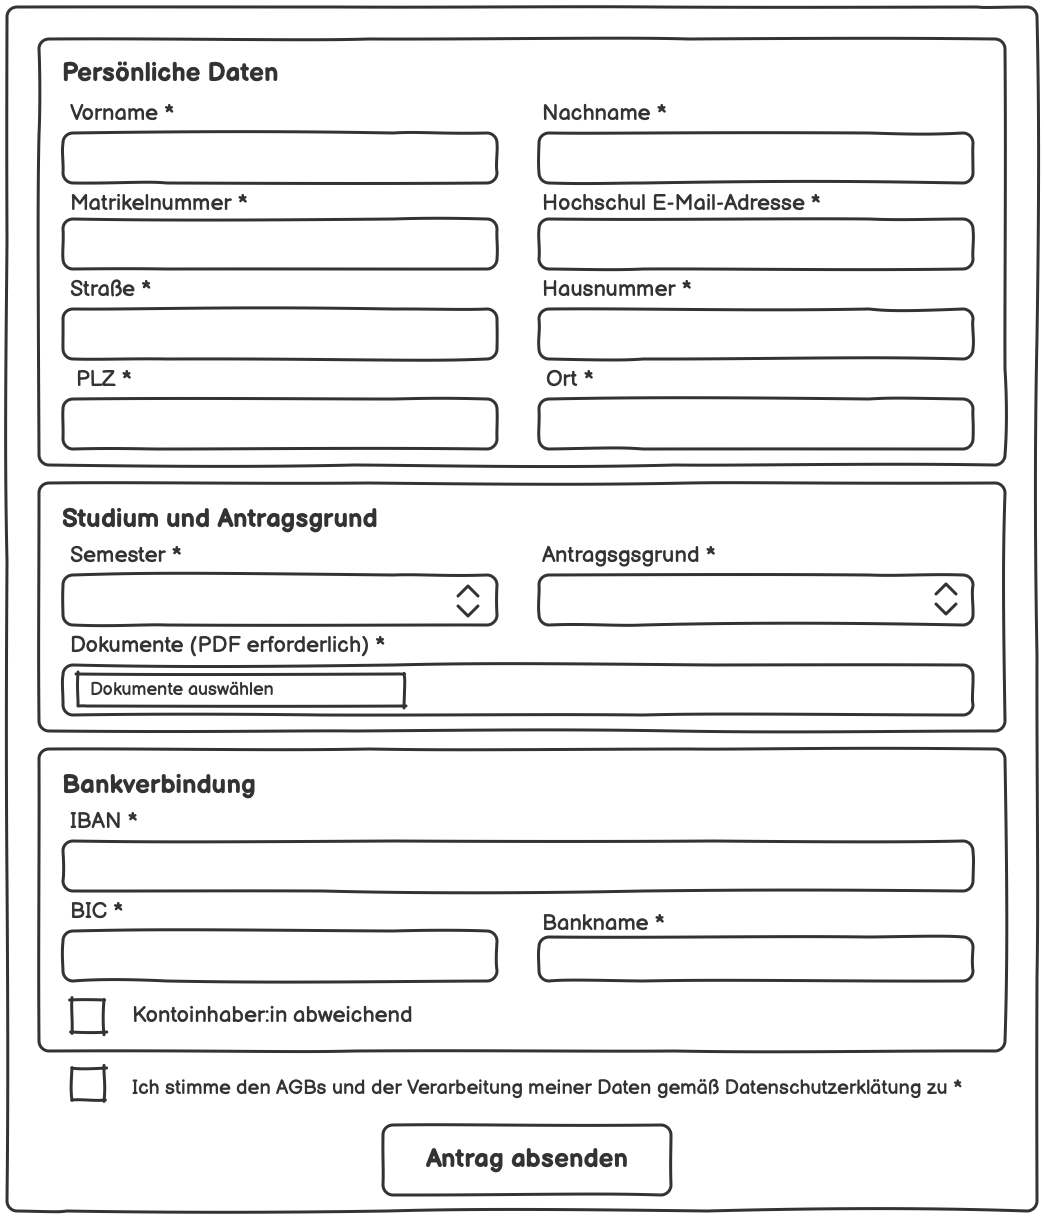
\includegraphics[width=0.9\textwidth]{Bilder/Antragsformular.png}
  \caption{User Interface des Antragsformulars}\label{fig:antragsformular}
\end{figure}

\section{Bearbeitungsportal}
Das Bearbeitungsportal für die Mirarbeitenden des Sozialbüros bildet den Kern der Lösung. Wenn der/die Nutzende die Webapplikation aufrufen, wird er/sie auf der ersten Seite aufgefordert, sich einzuloggen. Nach dem Login wird der/die Nutzende auf die Seite mit den zu bearbeitenden Anträgen weitergeleitet. Die eingegangenen Anträge sowie die Anträge, bei welchen Dokumente nachgefordert wurden, werden hier angezeigt. Abbildung~\ref{fig:aktuelleAnträge} zeigt eine mögliche Darstellung dieser Seite. Analog dazu soll es eine weitere Seite geben, auf welcher alle bewilligte, abgelehnten sowie archivierten Anträge angezeigt werden. Diese ist in Abbildung~\ref{fig:archivierteAnträge} dargestellt. 
\begin{figure}[htbp]
  \centering
  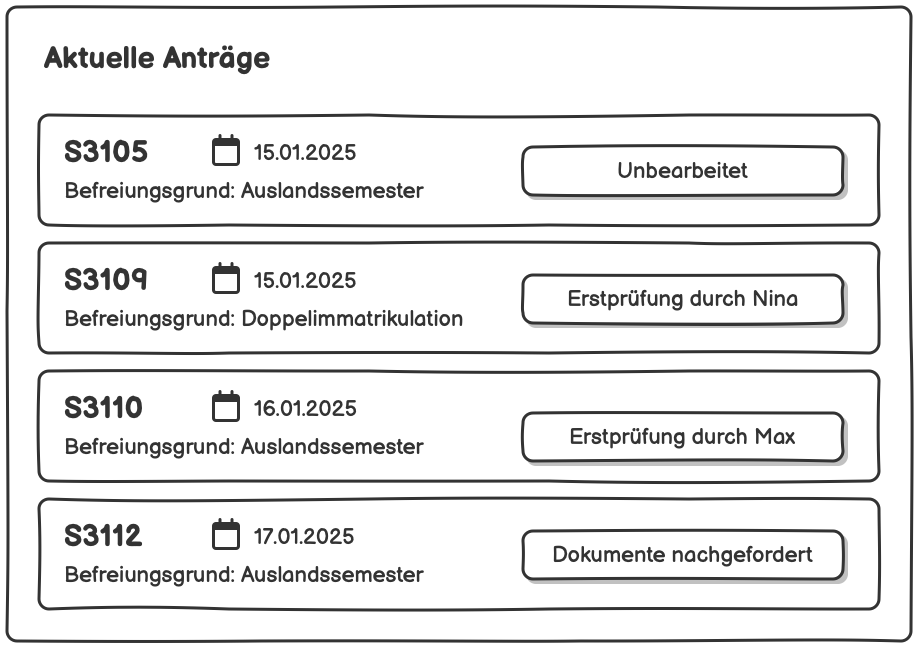
\includegraphics[width=0.9\textwidth]{Bilder/Aktuelle_Anträge.png}
  \caption{User Interface des Bearbeitungsortals auf der Seite Aktuelle Anträge}\label{fig:aktuelleAnträge}
\end{figure}

\begin{figure}[htbp]
  \centering
  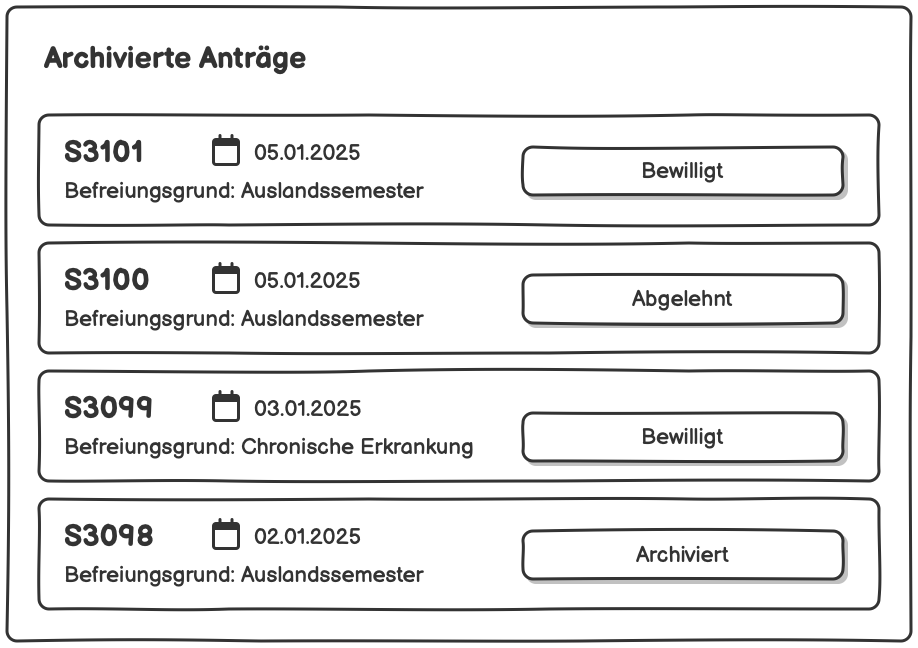
\includegraphics[width=0.9\textwidth]{Bilder/Archivierte_Anträge.png}
  \caption{User Interface des Bearbeitungsortals auf der Seite Archivierte Anträge}\label{fig:archivierteAnträge}
\end{figure}

% \begin{figure}
% \centering
% \begin{minipage}{.5\textwidth}
%   \centering
%   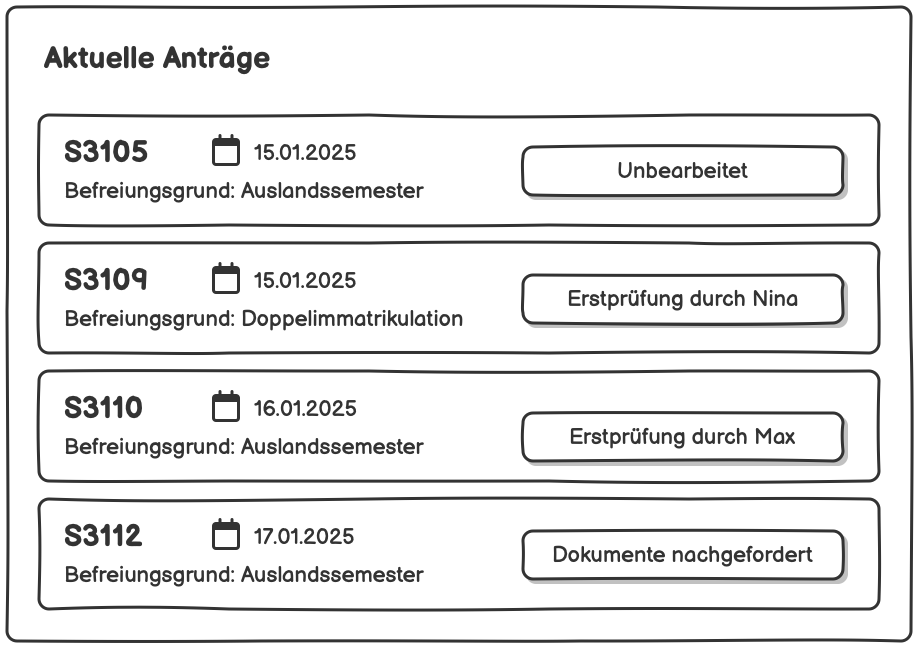
\includegraphics[width=0.9\linewidth]{Bilder/Aktuelle_Anträge.png}
%   \captionof{figure}{User Interface des Bearbeitungsortals auf der Seite \glqq{}Aktuelle Anträge\grqq{}}\label{fig:aktuelleAnträge}
% \end{minipage}%
% \begin{minipage}{.5\textwidth}
%   \centering
%   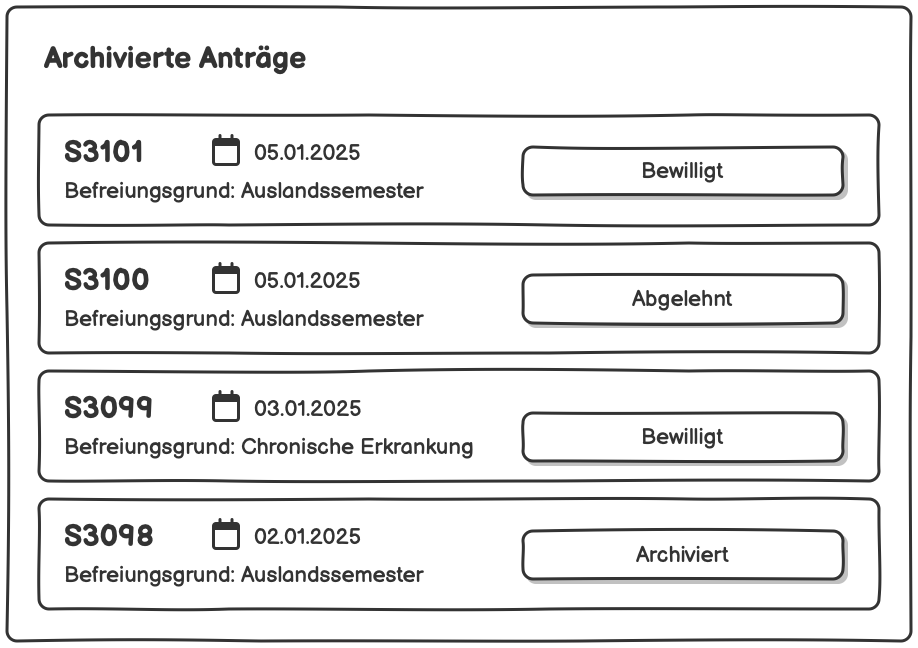
\includegraphics[width=0.9\linewidth]{Bilder/Archivierte_Anträge.png}
%   \captionof{figure}{User Interface des Bearbeitungsortals auf der Seite \glqq{}Archivierte Anträge\grqq{}}\label{fig:archivierteAnträge}
% \end{minipage}
% \end{figure}

Zur Bearbeitung eines Antrags muss die Detailansicht geöffnet werden (siehe Abbildung~\ref{fig:detailAnträge}). Auf dieser werden alle von dem/der Studierenden sowie die hochgeladenen Dokumente angezeigt. Die Daten werden auf Vollständigkeit von den Mitarbeitenden des Sozialbüros überprüft. Es muss eingetragen werden, wer den Antrag erstgeprüft und wer zweitgeprüft hat. Daraufhin kann über einen Button der Bewilligungs- oder Ablehnungsbescheid generiert werden. Es gibt außerdem die Möglichkeit den Status des Antrags auf \glqq{}Archiviert\grqq{}, \glqq{} Dokumente nachgefordert\grqq{} oder \glqq{}Zurückgezogen\grqq{}  zu setzen. Der/die Erstprüfende befindet den Antrag nach der Prüfung für bewilligt oder Abgelehnt. Der Status Ändert sich dadurch zu \glqq{}Erstprüfung durch xy\grqq{}. Ob er bewilligt oder abgelehnt wurde, erscheint neben dem Name des/der Erstprüfenden. Ein:e weitere:r Mitarbeitende führt daraufhin die Zweitprüfung durch. Bleibt die Entschiedung gleich, kann ein Bewilligungs- oder Ablehnungsbescheid erstellt werden und per Knopfdruck an den/die Studierende:n, sowie bei einer Bewilligung an das Finanzteam, versendet werden. Unterscheiden sich die beiden Entscheidungen der Mitarbeitenden, wird der Status des Antrags wieder auf \glqq{}Unbearbeitet\grqq{} gesetzt und die Entscheidung muss mündlich in Absprache getroffen werden. Der gesamte Prozess von Antragseinreichung durch das Online-Formular auf der \gls{asta} Website über die Bearbeitung des Antrags bis hin zum Versandt des Bescheids ist in Abbildung~\ref{fig:sollProzess} dargestellt.

\begin{figure}[htbp]
  \centering
  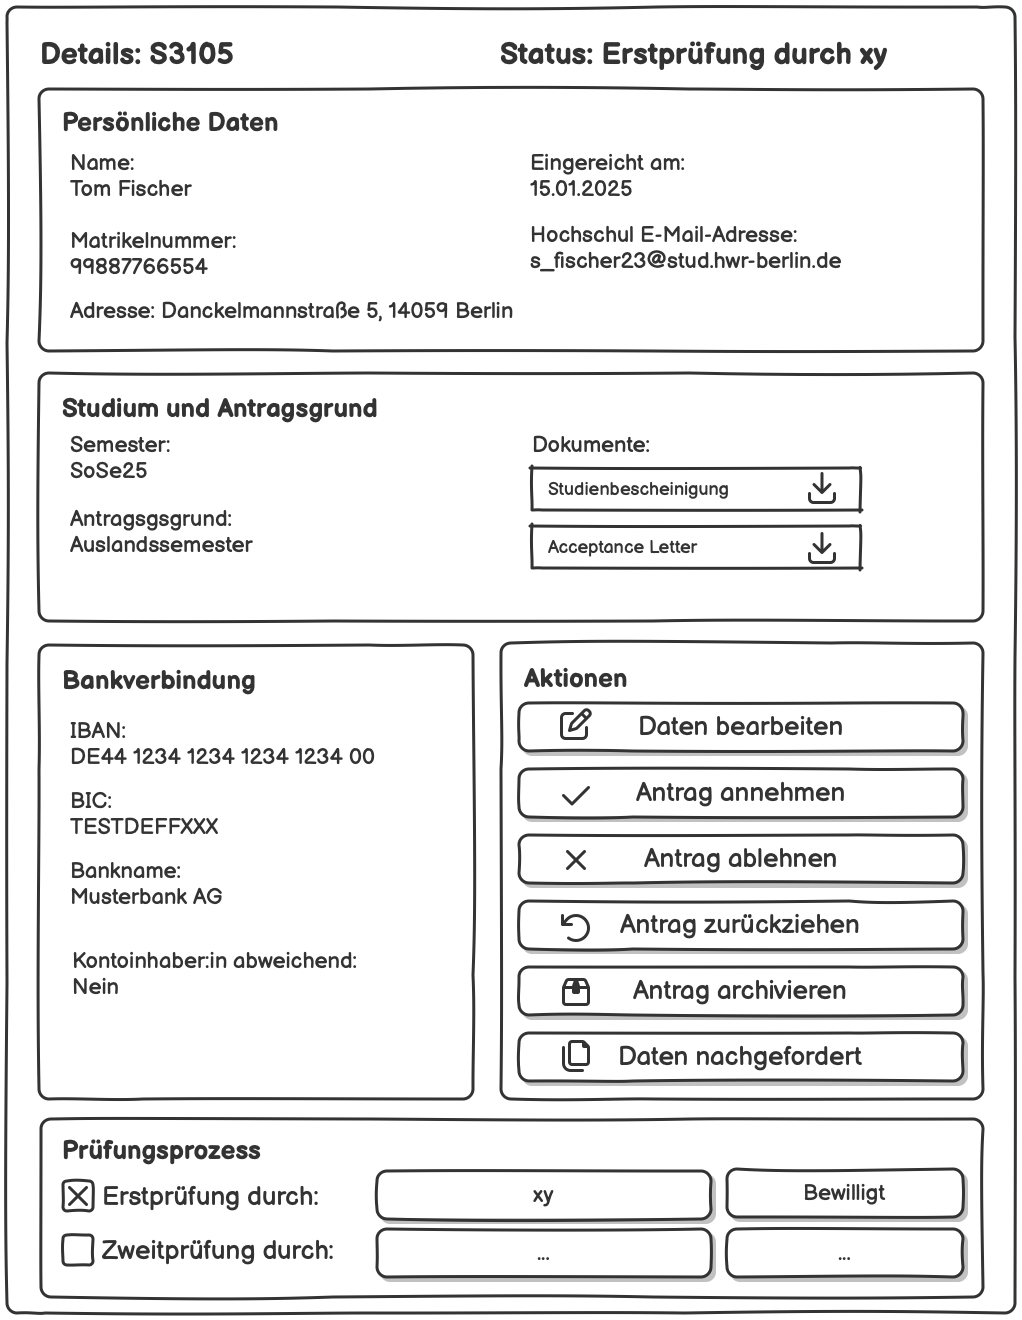
\includegraphics[width=0.8\textwidth]{Bilder/Detail_Antrag.png}
  \caption{Detailansicht eines Antrags}\label{fig:detailAnträge}
\end{figure}

\begin{figure}[htbp]
  \centering
  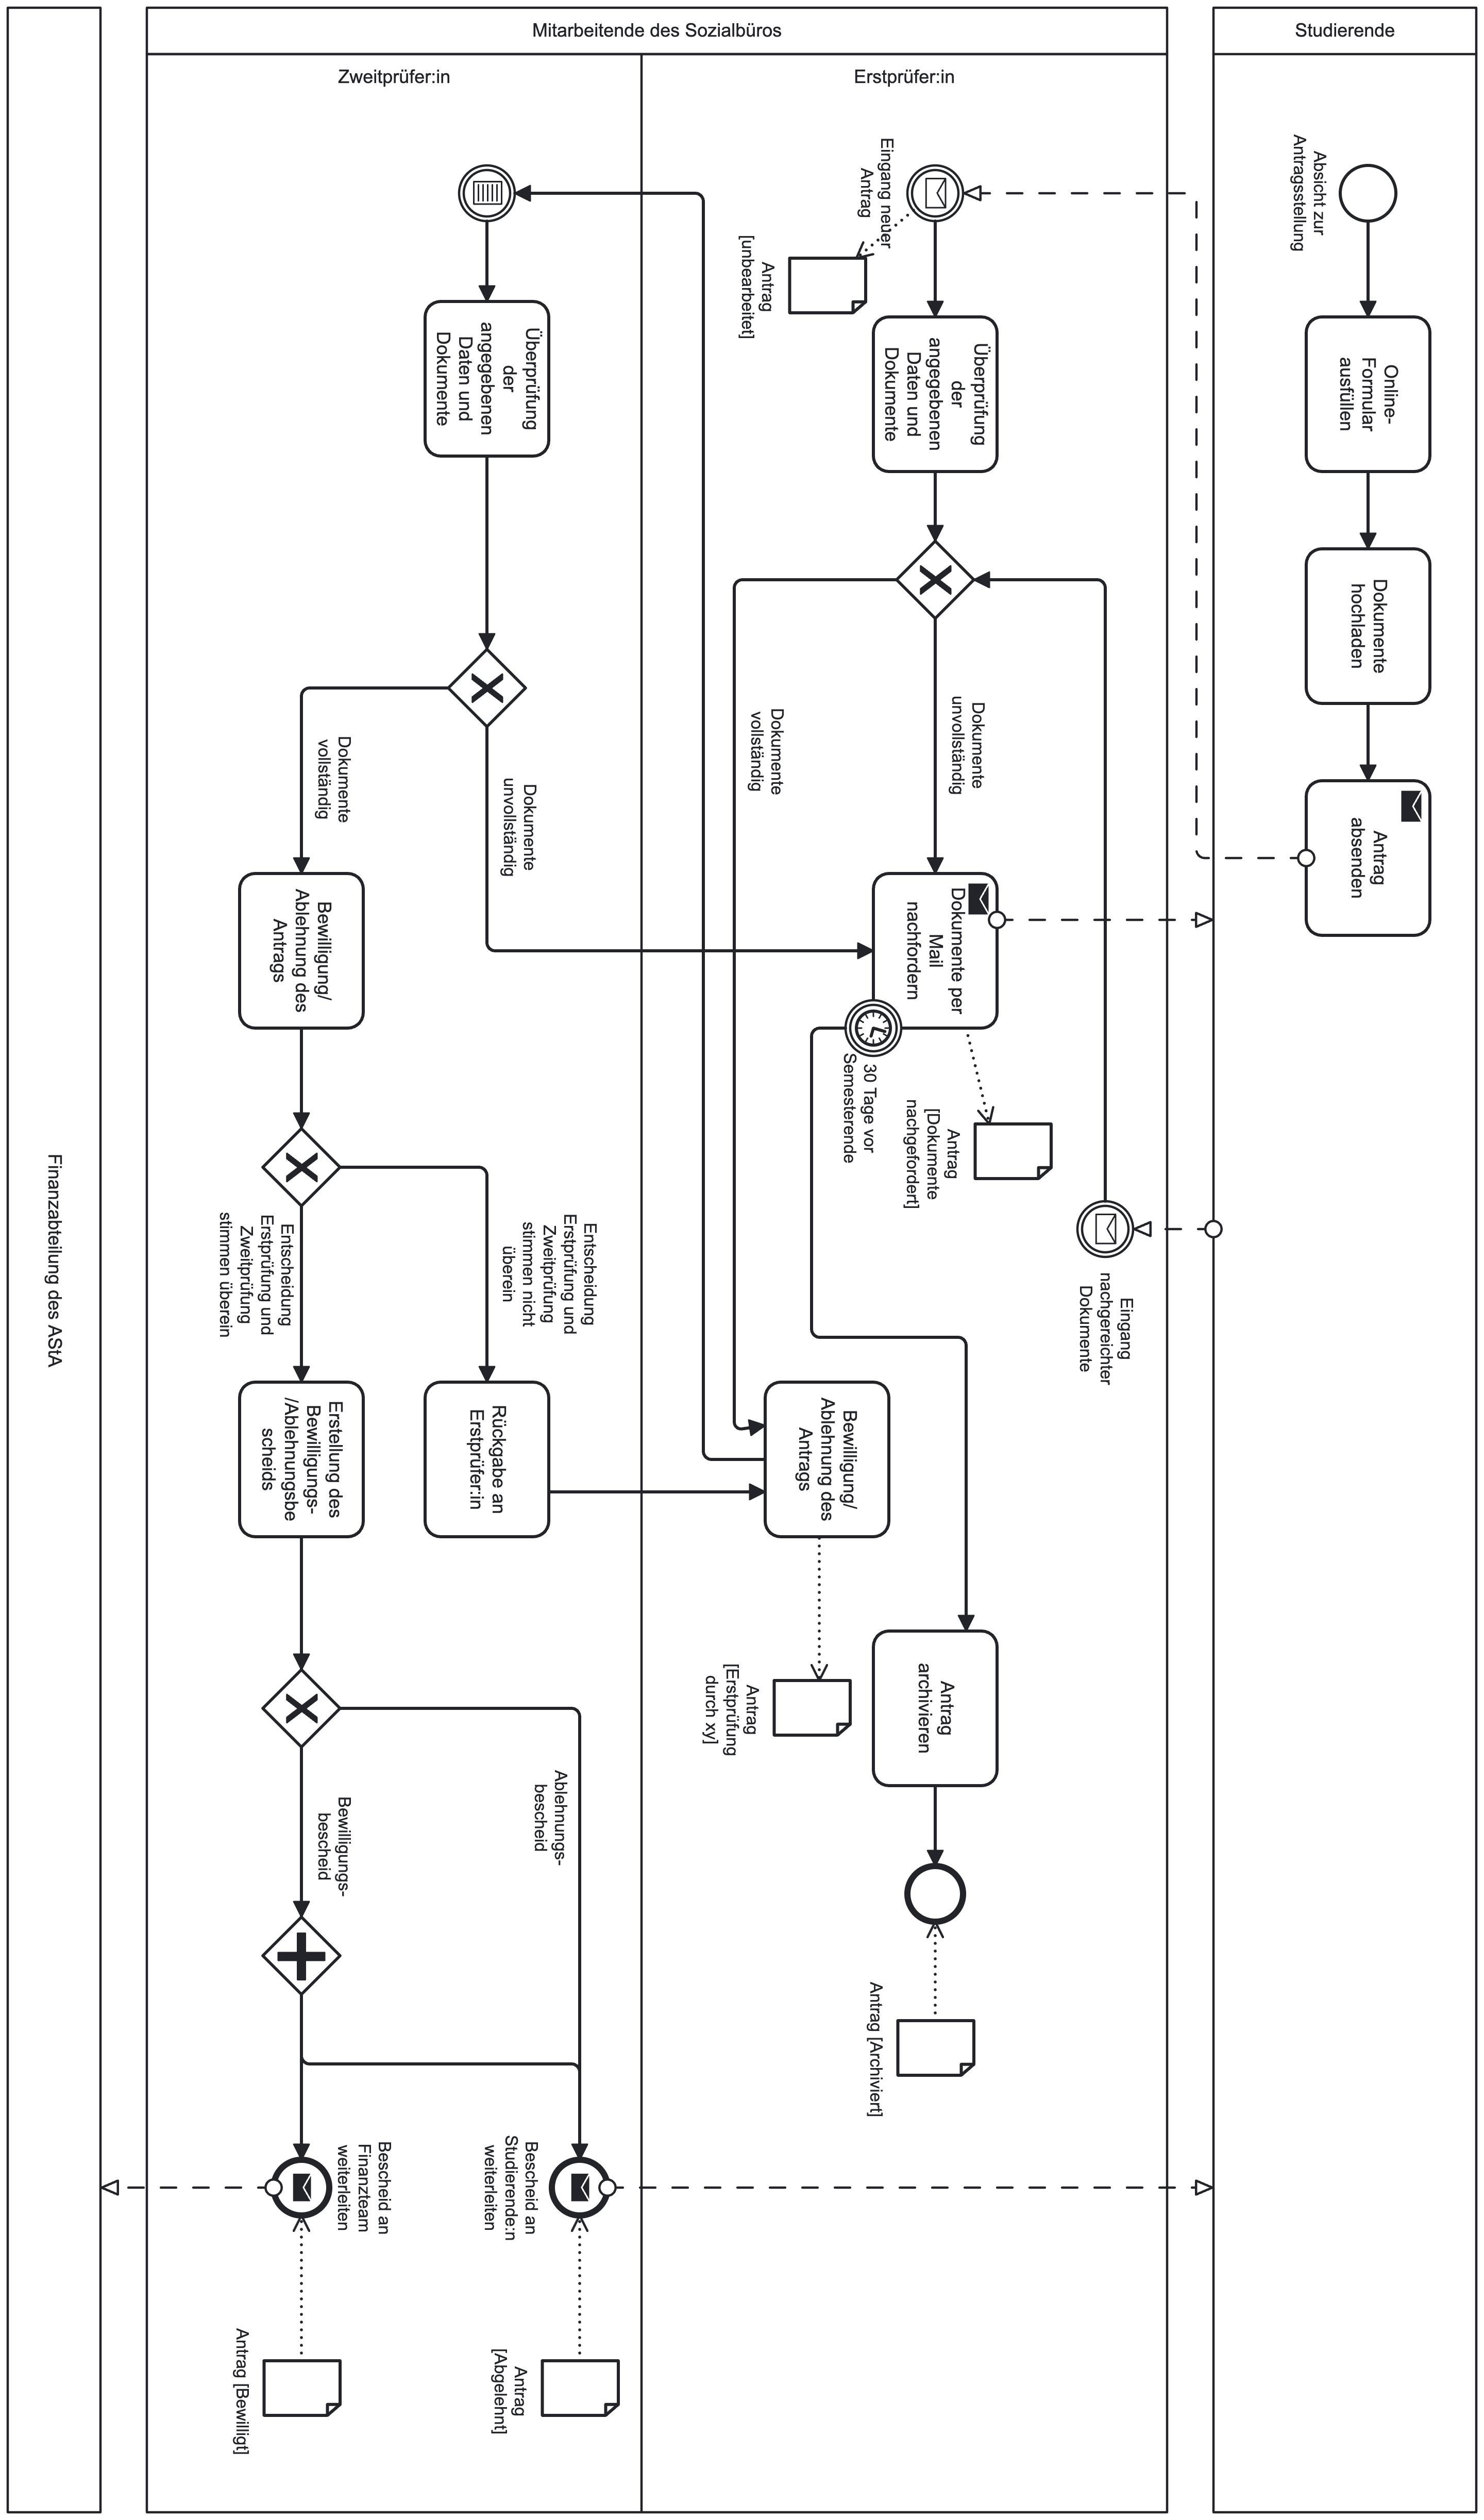
\includegraphics[width=0.9\textwidth]{Bilder/BPMNsollProzess.png}
  \caption{BPMN-SOLL-Model des Antragsprozesses}\label{fig:sollProzess}
\end{figure}

\section{Datenmodell}\label{sec:datenmodell}
Zum Aufbau einer Datenbankstruktur ist es sinnvoll, ein nach der Anforderungsanalyse ein Datenbankschema zu entwickeln. Ein solches konzeptionelles Schema ist das \gls{erm}. Als Entität ist ein Objekt zu verstehen, welches verschidene Charakteristika haben kann. Mehrere Entitäten mit den gleichen Eigenschaften werden als Entitätsmenge zusammengefasst. Bei einer Entitätsmenge ist es deshalb notwendig, ein Attribut zu bestimmen, welches die Entitäten voneinander unterscheidet. Das kann Beispielsweise eine ID sein. Diese Entitätsmengen sind durch Beziehungen verknüpft, welche wiederum selbst Merkmale haben können. Ein solches \gls{erm} kann dann auf eine Datenbank abgebildet werden. \VglZitat{SQL}{29 ff.} Ein \gls{erm} zum Antragsprozess ist in Abbildung~\ref{fig:erm} dargestellt. Es gibt folgende Entitätsmengen: 
\begin{description}
  \item[Student:in:] Das ist die Person, welche den Antrag stellt. Neben einer eindeutigen ID werden auch die personenbezogenen Daten als Attribute gespeichert. Eine Person kann pro Semester nur einen Antrag stellen. 
  \item[Antrag:] Der Antrag ist das Kernstück. Es werden das Semester, Antragsgrund und Antragsdatum sowie die Bankdaten gespeichert. Ein Antrag beinhaltet mehrere Dokumente und er kann verschiedene Bearbeitungszustände während des Prozesses annehmen. 
  \item[Mitarbeiter:in:] Hierbei handelt es sich um die Personen, die einen Antrag prüfen, den Status ändern und den dazugehörigen Bewilligungs- oder Ablehnungsbescheid erstellen. 
  \item[Bearbeitungshistorie:] Die Bearbeitungshistorie dokumentiert die Änderungen eines Antrags während des Prüfprozesses. Jede Änderung des Status wird mit dem Änderungsdatum sowie dem/der Mitarbeiter:in festgehalten, um den Prozess nachvollziehbar zu machen. 
  \item[Bescheid:] Ein Antrag kann bewilligt oder abgelehnt werden (muss er aber nicht). Geschieht das, wird ein Bescheid von einem/einer Mitarbeitenden erstellt. Jeder Antrag kann nur einen Bescheid haben.   
\end{description}

\begin{figure}[htbp]
  \centering
  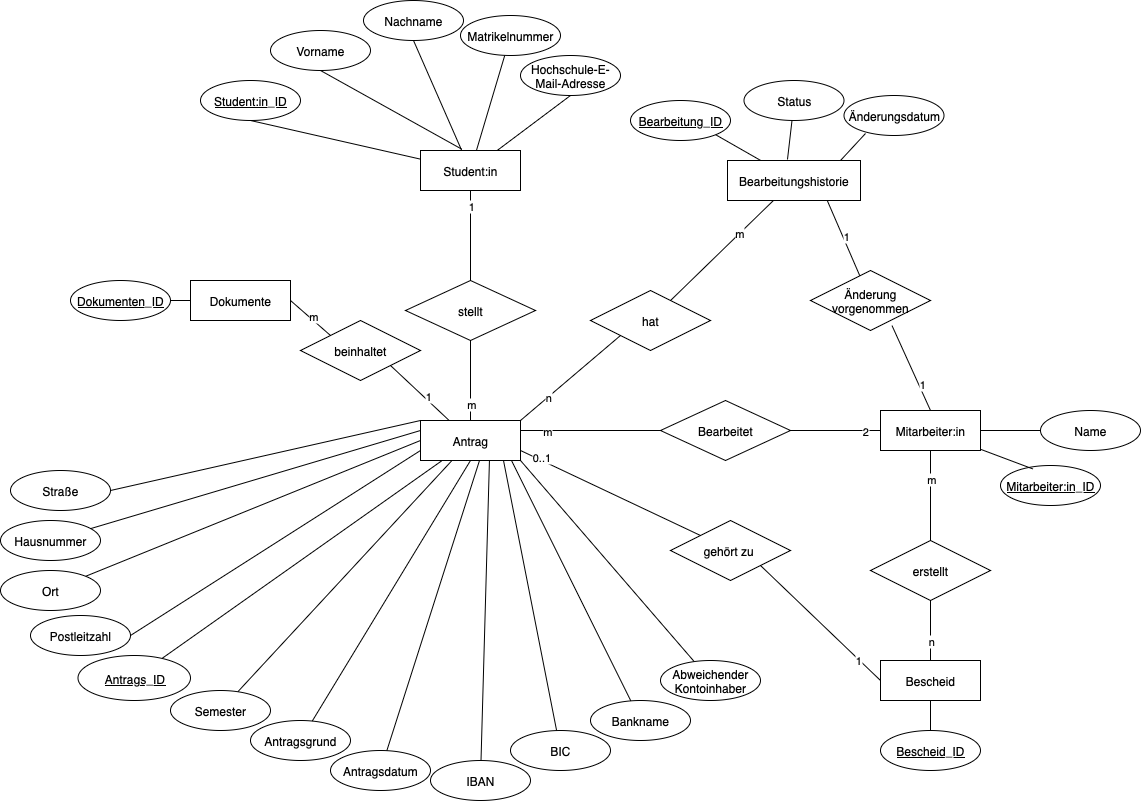
\includegraphics[width=1\textwidth]{Bilder/ERM.png}
  \caption{\gls{erm} des Antragsprozesses}\label{fig:erm}
\end{figure}

Das Relationsmodell beschreibt Daten und ihre Beziehungen zueinander in Form von Tabellen. Daraus hervorgehend entstanden relationale Datenbanken. Relation mein hier nicht, wie umgangssprachlich  verstanden, eine \glqq{}Beziehung\grqq{}, sondern eine Teilmenge aller möglichen Kombinationen der Werte der Attribute, wobei eine Relation als $R$ und die Mengen der Werte der Attribute mit $D_n$ bezeichnet werden.

Mathematisch lässt sich das so ausdrücken:
\[
R \subseteq D_1 \times D_2 \times \dots \times D_n
\]
Eine Relation ist auch eine Menge sogenannter Tupel. Ein Tupel $r$ ist eine Menge konkreter Datenwerte, also Ausprägungen der Attribute $D_i$. Die Menge aller Tupel einer Relation lässt sich wie folgt darstellen:
\[
R = \{ r_1, r_2, \dots, r_m \}
\]
Augrund des mathematischen Mengenbegriffs, darf ein Tupel nicht mehrfach vorkommen. Deshalb ist es sinnvll eine eindeutiges Attribut wie eine ID als Primärschlüssel hinzuzufügen. \VglZitat{SQL}{41 f.}

Um das im Vorhinein erstellte \gls{erm} in ein relationales Datenbankschema umzuwandeln, müssen verschiedene Abbildungsregeln beachtet werden. Regel 1 besagt, dass jede Entitätsmenge einen Primärschlüssel, also ein eindeutiges Attribut aufweisen muss. Das sind im Beispielmodell \ref{fig:erm} verschiedene IDs. Die zweite Regel besagt, dass auch jede Beziehungsmenge eine eigene Tabelle haben kann. Diese Tabelle muss keinen eigenen Primärschlüssel haben, da dieser aus den Fremdschlüsseln der Entitätsmengen gebildet werden kann. \VglZitat{SQL}{49 f.} ??? ist das hier sinnvoll???

\section{Technische Umsetzung}\label{sec:technischeUmsetzung}
Die Webanwendung soll auf der Website des \gls{asta} erscheinen. Die aktuelle Website basiert auf Wordpress. 